% Relatório final — RotaGrafo (TP de Grafos, tema 10)
% Template SBC: copie sbc-template.sty e sbc.bst do Overleaf
% (https://www.overleaf.com/latex/templates/sbc-conferences-template/blbxwjwzdngr)
% para esta pasta, ou crie o projeto no Overleaf a partir do template e cole este arquivo.
%
% Legenda dos comentários:  % [DUPLA X] = seção sob responsabilidade da dupla X
%                           % TODO      = falta preencher

\documentclass[12pt]{article}

\usepackage{sbc-template}
\usepackage{graphicx,url}
\usepackage[utf8]{inputenc}
\usepackage[brazil]{babel}
\usepackage{amsmath}
\usepackage{booktabs}
\usepackage{listings}
\usepackage{float}  % permite [H]: figura fica exatamente onde foi escrita

\lstset{basicstyle=\ttfamily\footnotesize, breaklines=true, frame=single}

\sloppy

\title{RotaGrafo: Roteamento e Carga de Veículos em\\Centros Logísticos com Grafos}

% TODO: nomes completos
\author{Zaine\inst{1}, Bruna\inst{1}, Kethellen\inst{1}, Rafael\inst{1}, Filipe Quaresma Pereira\inst{1}, Vitor\inst{1}}

% TODO: instituição
\address{Instituição -- Curso -- Cidade, UF -- Brasil}

\begin{document}

\maketitle

% [DUPLA 3] — revisar ao final, quando os resultados estiverem prontos
\begin{abstract}
This work presents RotaGrafo, a tool for planning delivery routes from a logistics
center. The delivery network is modeled as a weighted graph whose vertices are the
depot and the customers, and whose edges carry distance and travel time. Routes are
built with the Nearest Neighbor and Clarke-Wright heuristics and refined with 2-opt,
respecting vehicle capacity, time windows and delivery priority. A web interface with
an interactive map allows configuring the fleet, visualizing the routes and comparing
algorithms. % TODO: principal resultado numérico
\end{abstract}

\begin{resumo}
Este trabalho apresenta o RotaGrafo, uma ferramenta para o planejamento de rotas de
entrega a partir de um centro logístico. A rede de entregas é modelada como um grafo
ponderado cujos vértices são o depósito e os clientes e cujas arestas carregam
distância e tempo de deslocamento. As rotas são construídas com as heurísticas do
Vizinho Mais Próximo e de Clarke-Wright e refinadas com 2-opt, respeitando a
capacidade dos veículos, as janelas de tempo e a prioridade das entregas. Uma
interface web com mapa interativo permite configurar a frota, visualizar as rotas e
comparar os algoritmos. % TODO: principal resultado numérico
\end{resumo}

% =====================================================================
\section{Introdução}
% [DUPLA 3]

A distribuição de mercadorias é uma das etapas mais custosas da cadeia logística.
Em um centro de distribuição urbano, uma frota limitada de veículos precisa atender
dezenas ou centenas de clientes por dia. Cada veículo tem uma capacidade de carga
máxima, cada cliente tem um horário em que pode receber a entrega e alguns pedidos
são mais urgentes que outros. Decidir quais clientes cada veículo atende, e em que
ordem, afeta diretamente a distância percorrida, o consumo de combustível, o número
de veículos necessários e a quantidade de entregas atrasadas.

Esse cenário corresponde ao \textit{Problema de Roteamento de Veículos} (VRP), em
especial às variantes com restrição de capacidade (CVRP) e com janelas de tempo
(VRPTW)~\cite{toth2014vehicle,solomon1987algorithms}. O VRP generaliza o Problema do
Caixeiro Viajante e é NP-difícil. Por isso, instâncias de tamanho realista são
resolvidas na prática com heurísticas, que encontram boas soluções em tempo
polinomial sem garantia de otimalidade.

A estrutura central do problema é um grafo: os locais de entrega são vértices e os
deslocamentos entre eles são arestas ponderadas. Este trabalho desenvolve o
\textbf{RotaGrafo}, uma ferramenta que:
\begin{itemize}
  \item modela a rede de entregas como um grafo ponderado implementado do zero, sem
        bibliotecas prontas;
  \item calcula caminhos mínimos entre os pontos com o algoritmo de
        Dijkstra~\cite{dijkstra1959note};
  \item constrói rotas com as heurísticas do Vizinho Mais Próximo e de
        Clarke-Wright~\cite{clarke1964scheduling} e as refina com
        2-opt~\cite{croes1958method};
  \item apresenta os resultados em uma interface web com mapa interativo, métricas e
        comparação entre algoritmos.
\end{itemize}

O restante do artigo está organizado da seguinte forma: a
Seção~\ref{sec:modelagem} apresenta a modelagem do grafo e os dados utilizados; a
Seção~\ref{sec:algoritmos} descreve os algoritmos e suas complexidades; a
Seção~\ref{sec:arquitetura} mostra a arquitetura da ferramenta e a interface; a
Seção~\ref{sec:resultados} analisa os resultados e o desempenho; a
Seção~\ref{sec:limitacoes} discute as limitações; e a
Seção~\ref{sec:conclusao} conclui o trabalho.

% =====================================================================
\section{Modelagem do Problema}\label{sec:modelagem}
% [DUPLA 1]

% TODO (Dupla 1):
%  - definição formal: G = (V, E), V = {0 (depósito), 1..n (clientes)}, pesos d(u,v) e t(u,v)
%  - atributos de cada vértice: demanda q_i, janela [a_i, b_i], prioridade p_i
%  - justificativa da representação (lista de adjacência x matriz; grafo completo x rede viária)
%  - diagramas UML: classes, casos de uso, atividades (figuras)
%  - descrição da base de dados (origem/Kaggle, tamanho, tratamento)

\subsection{Definição formal}
% TODO

\subsection{Diagramas UML}
% TODO
% \begin{figure}[ht]
%   \centering
%   \includegraphics[width=.9\textwidth]{figuras/uml-classes.png}
%   \caption{Diagrama de classes.}
%   \label{fig:uml-classes}
% \end{figure}

\subsection{Base de dados}
% TODO

% =====================================================================
\section{Algoritmos}\label{sec:algoritmos}
% [DUPLA 2] (Dijkstra: Dupla 1)

% TODO: para cada algoritmo -> ideia, pseudocódigo curto, como trata capacidade /
% janela / prioridade, e complexidade de tempo e espaço.

\subsection{Caminhos mínimos: Dijkstra}
% TODO (Dupla 1)

\subsection{Vizinho Mais Próximo}
% TODO

\subsection{Clarke-Wright (\textit{Savings})}
% TODO

\subsection{Melhoria local: 2-opt}
% TODO

\subsection{Resumo das complexidades}
% TODO: preencher a tabela
\begin{table}[ht]
\centering
\caption{Complexidade dos algoritmos implementados ($n$ = número de vértices).}
\label{tab:complexidade}
\begin{tabular}{lcc}
\toprule
Algoritmo & Tempo & Espaço \\
\midrule
Dijkstra (heap binário)      & $O((V+E)\log V)$ & $O(V)$ \\
Vizinho Mais Próximo         & $O(n^2)$         & $O(n)$ \\
Clarke-Wright                & $O(n^2 \log n)$  & $O(n^2)$ \\
2-opt (por iteração)         & $O(n^2)$         & $O(n)$ \\
\bottomrule
\end{tabular}
\end{table}

% =====================================================================
\section{Arquitetura e Interface}\label{sec:arquitetura}
% [DUPLA 3]

\subsection{Arquitetura}

A ferramenta segue uma arquitetura cliente-servidor em três camadas
(Figura~\ref{fig:arquitetura}):
\begin{enumerate}
  \item \textbf{Núcleo de grafos} (Python): a estrutura do grafo, a leitura dos
        dados e os algoritmos de roteirização, implementados sem bibliotecas de grafos;
  \item \textbf{API REST} (Flask): expõe o núcleo por meio de rotas HTTP com
        respostas em JSON e controla o acesso por login e sessão;
  \item \textbf{Interface web} (HTML, CSS e JavaScript com Leaflet): consome a API e
        apresenta os resultados sobre um mapa do OpenStreetMap.
\end{enumerate}

\begin{figure}[H]
  \centering
  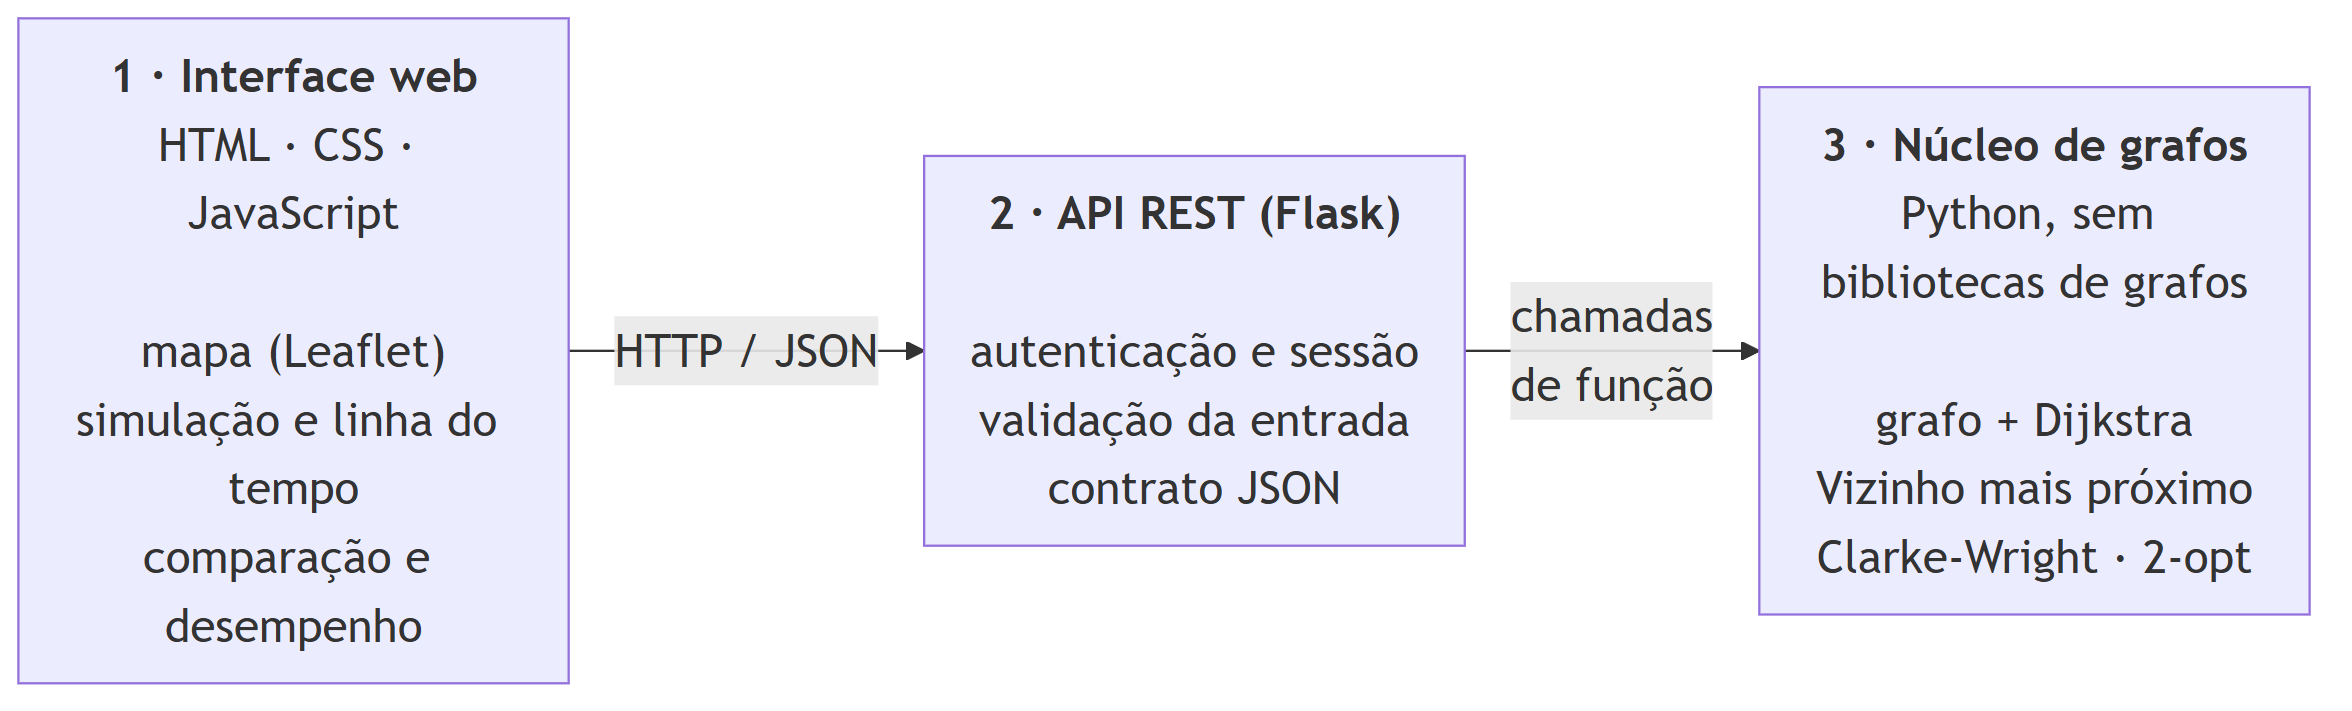
\includegraphics[width=\textwidth]{figuras/arquitetura.png}
  \caption{Arquitetura do RotaGrafo em três camadas.}
  \label{fig:arquitetura}
\end{figure}

A comunicação entre as camadas segue um contrato JSON fixo
(Tabela~\ref{tab:api}). Esse contrato permitiu que as três duplas trabalhassem em
paralelo: enquanto o núcleo era implementado, a interface foi construída sobre dados
de exemplo no mesmo formato e depois conectada ao código real trocando apenas as
quatro linhas do ponto de integração em \texttt{src/api/app.py}.

\begin{table}[ht]
\centering
\caption{Rotas da API.}
\label{tab:api}
\begin{tabular}{lp{9cm}}
\toprule
Rota & Descrição \\
\midrule
\texttt{GET /api/grafo}       & Vértices (posição, demanda, janela, prioridade) e arestas (distância, tempo). \\
\texttt{GET /api/algoritmos}  & Algoritmos disponíveis. \\
\texttt{POST /api/rotas}      & Recebe frota, capacidade, algoritmo e uso do 2-opt; devolve as rotas, os horários de chegada, os clientes não atendidos, as métricas e o tempo de execução. \\
\texttt{GET /api/desempenho}  & Recebe uma lista de tamanhos de grafo e devolve o tempo de execução de cada algoritmo em cada tamanho. \\
\texttt{POST /api/auth/login} & Recebe e-mail e senha e inicia a sessão. \\
\texttt{POST /api/auth/registrar} & Cria uma conta e inicia a sessão. \\
\texttt{POST /api/auth/logout} & Encerra a sessão. \\
\bottomrule
\end{tabular}
\end{table}

\subsection{Validação do contrato}

Para garantir que a integração entre as partes não quebrasse a interface, foi criado
um validador (\texttt{src/api/contrato.py}) com testes automatizados. Ele verifica,
para várias combinações de frota, capacidade e algoritmo, que:
\begin{itemize}
  \item toda rota começa e termina no depósito;
  \item nenhuma rota excede a capacidade do veículo;
  \item nenhum cliente é visitado mais de uma vez;
  \item todo cliente aparece em exatamente uma rota ou na lista de não atendidos;
  \item o número de rotas não passa do número de veículos disponíveis.
\end{itemize}

\subsection{Testes de corretude}

Os testes de contrato conferem o formato das respostas, mas não se os valores estão
certos. Por isso, um segundo conjunto de testes (\texttt{tests/test\_corretude.py})
recalcula os resultados de forma independente. Ele implementa uma versão de
referência do Dijkstra, conferida contra o algoritmo de Floyd-Warshall, e a usa para
verificar, em várias instâncias e configurações de frota, que:
\begin{itemize}
  \item o grafo é conexo a partir do depósito e não tem laços nem arestas repetidas;
  \item a distância de cada rota é igual à soma dos caminhos mínimos entre paradas
        consecutivas;
  \item nenhum veículo chega a um cliente antes do que o caminho mínimo em tempo
        permite;
  \item cada entrega começa em $\max(\text{chegada}, a_i)$, ou seja, o veículo
        espera a janela abrir, mas não espera sem necessidade, e é marcada como
        atrasada exatamente quando começa depois de $b_i$;
  \item as métricas totais são a soma das rotas e a ocupação é $\text{carga}/Q$;
  \item com frota suficiente, nenhum cliente fica sem atendimento;
  \item em instâncias pequenas (5 a 7 clientes), nenhuma solução é mais curta que o
        ciclo ótimo calculado por força bruta, o que denunciaria um erro no cálculo
        das distâncias.
\end{itemize}

Dois testes adicionais avaliam a qualidade das heurísticas: o 2-opt nunca deve
aumentar a distância total, e o Clarke-Wright com 2-opt deve ficar a no máximo 25\%
do ótimo nas instâncias pequenas.
% TODO (Duplas 1 e 2): confirmar que esses dois testes passam com o código real

\subsection{Controle de acesso}

O acesso à ferramenta exige login. Sem uma sessão válida, as páginas redirecionam
para a tela de login e as rotas da API respondem com o código HTTP 401. As senhas
nunca são armazenadas: o servidor guarda apenas o \textit{hash} gerado pela
biblioteca Werkzeug. A sessão fica em um \textit{cookie} \texttt{HttpOnly}, que pode
durar 30 dias quando o usuário marca a opção ``Manter conectado''. Para dificultar
ataques de força bruta, cinco tentativas erradas seguidas para o mesmo e-mail e
endereço IP bloqueiam o login por 15 minutos, e cada endereço IP pode criar no máximo
10 contas por hora.

\subsection{Interface}

A interface (Figura~\ref{fig:tela-principal}) é dividida em um painel lateral com
três abas (Rotas, Comparação e Desempenho), um mapa e uma linha do tempo. Suas
funcionalidades são:
\begin{itemize}
  \item \textbf{Cenário}: número de vértices e arestas, demanda total, clientes de
        alta prioridade e uma estimativa do número mínimo de veículos
        ($\lceil \sum q_i / Q \rceil$). As arestas do grafo podem ser exibidas
        sobre o mapa;
  \item \textbf{Configuração}: número de veículos, capacidade, algoritmo e uso do 2-opt;
  \item \textbf{Rotas}: cada veículo é desenhado com uma cor, e as cores seguem uma
        paleta validada para daltonismo. Cada rota tem um cartão com distância,
        tempo, ocupação da carga e lista de entregas. Clicar em uma rota a destaca
        no mapa e na linha do tempo;
  \item \textbf{Simulação do dia}: um controle de reprodução anima os veículos
        percorrendo as rotas conforme os horários calculados. Os clientes mudam de
        estado (aguardando, em atendimento, entregue no prazo, entregue com atraso)
        e uma barra permite ir a qualquer horário
        (Figura~\ref{fig:tela-simulacao});
  \item \textbf{Linha do tempo}: um diagrama de Gantt com uma linha por veículo
        mostra as viagens, as esperas pela abertura da janela e as entregas.
        Entregas atrasadas são destacadas e, ao passar o mouse sobre uma entrega,
        a janela de tempo do cliente aparece ao fundo. Assim, as restrições de
        tempo do VRPTW ficam visíveis de forma direta;
  \item \textbf{Comparação}: executa todas as combinações de algoritmo, com e sem
        2-opt, e mostra uma tabela e um gráfico de barras com a melhor configuração
        destacada (Figura~\ref{fig:tela-comparacao});
  \item \textbf{Desempenho}: mede o tempo de execução dos algoritmos para grafos
        de vários tamanhos e o exibe em um gráfico de linhas, o que permite
        confrontar o comportamento empírico com a complexidade teórica
        (Seção~\ref{sec:resultados});
  \item \textbf{Guia de uso}: um tour interativo, exibido no primeiro acesso,
        destaca cada parte da tela e explica como usá-la;
  \item \textbf{Exportação}: salva o resultado em JSON para análise posterior.
\end{itemize}

Os diagramas de componentes, de sequência e de estados da interface estão
nas Figuras~\ref{fig:uml-componentes}, \ref{fig:uml-sequencia} e
\ref{fig:uml-estados}.

% Figuras geradas a partir de docs/diagramas.md (Mermaid).
\begin{figure}[H]
  \centering
  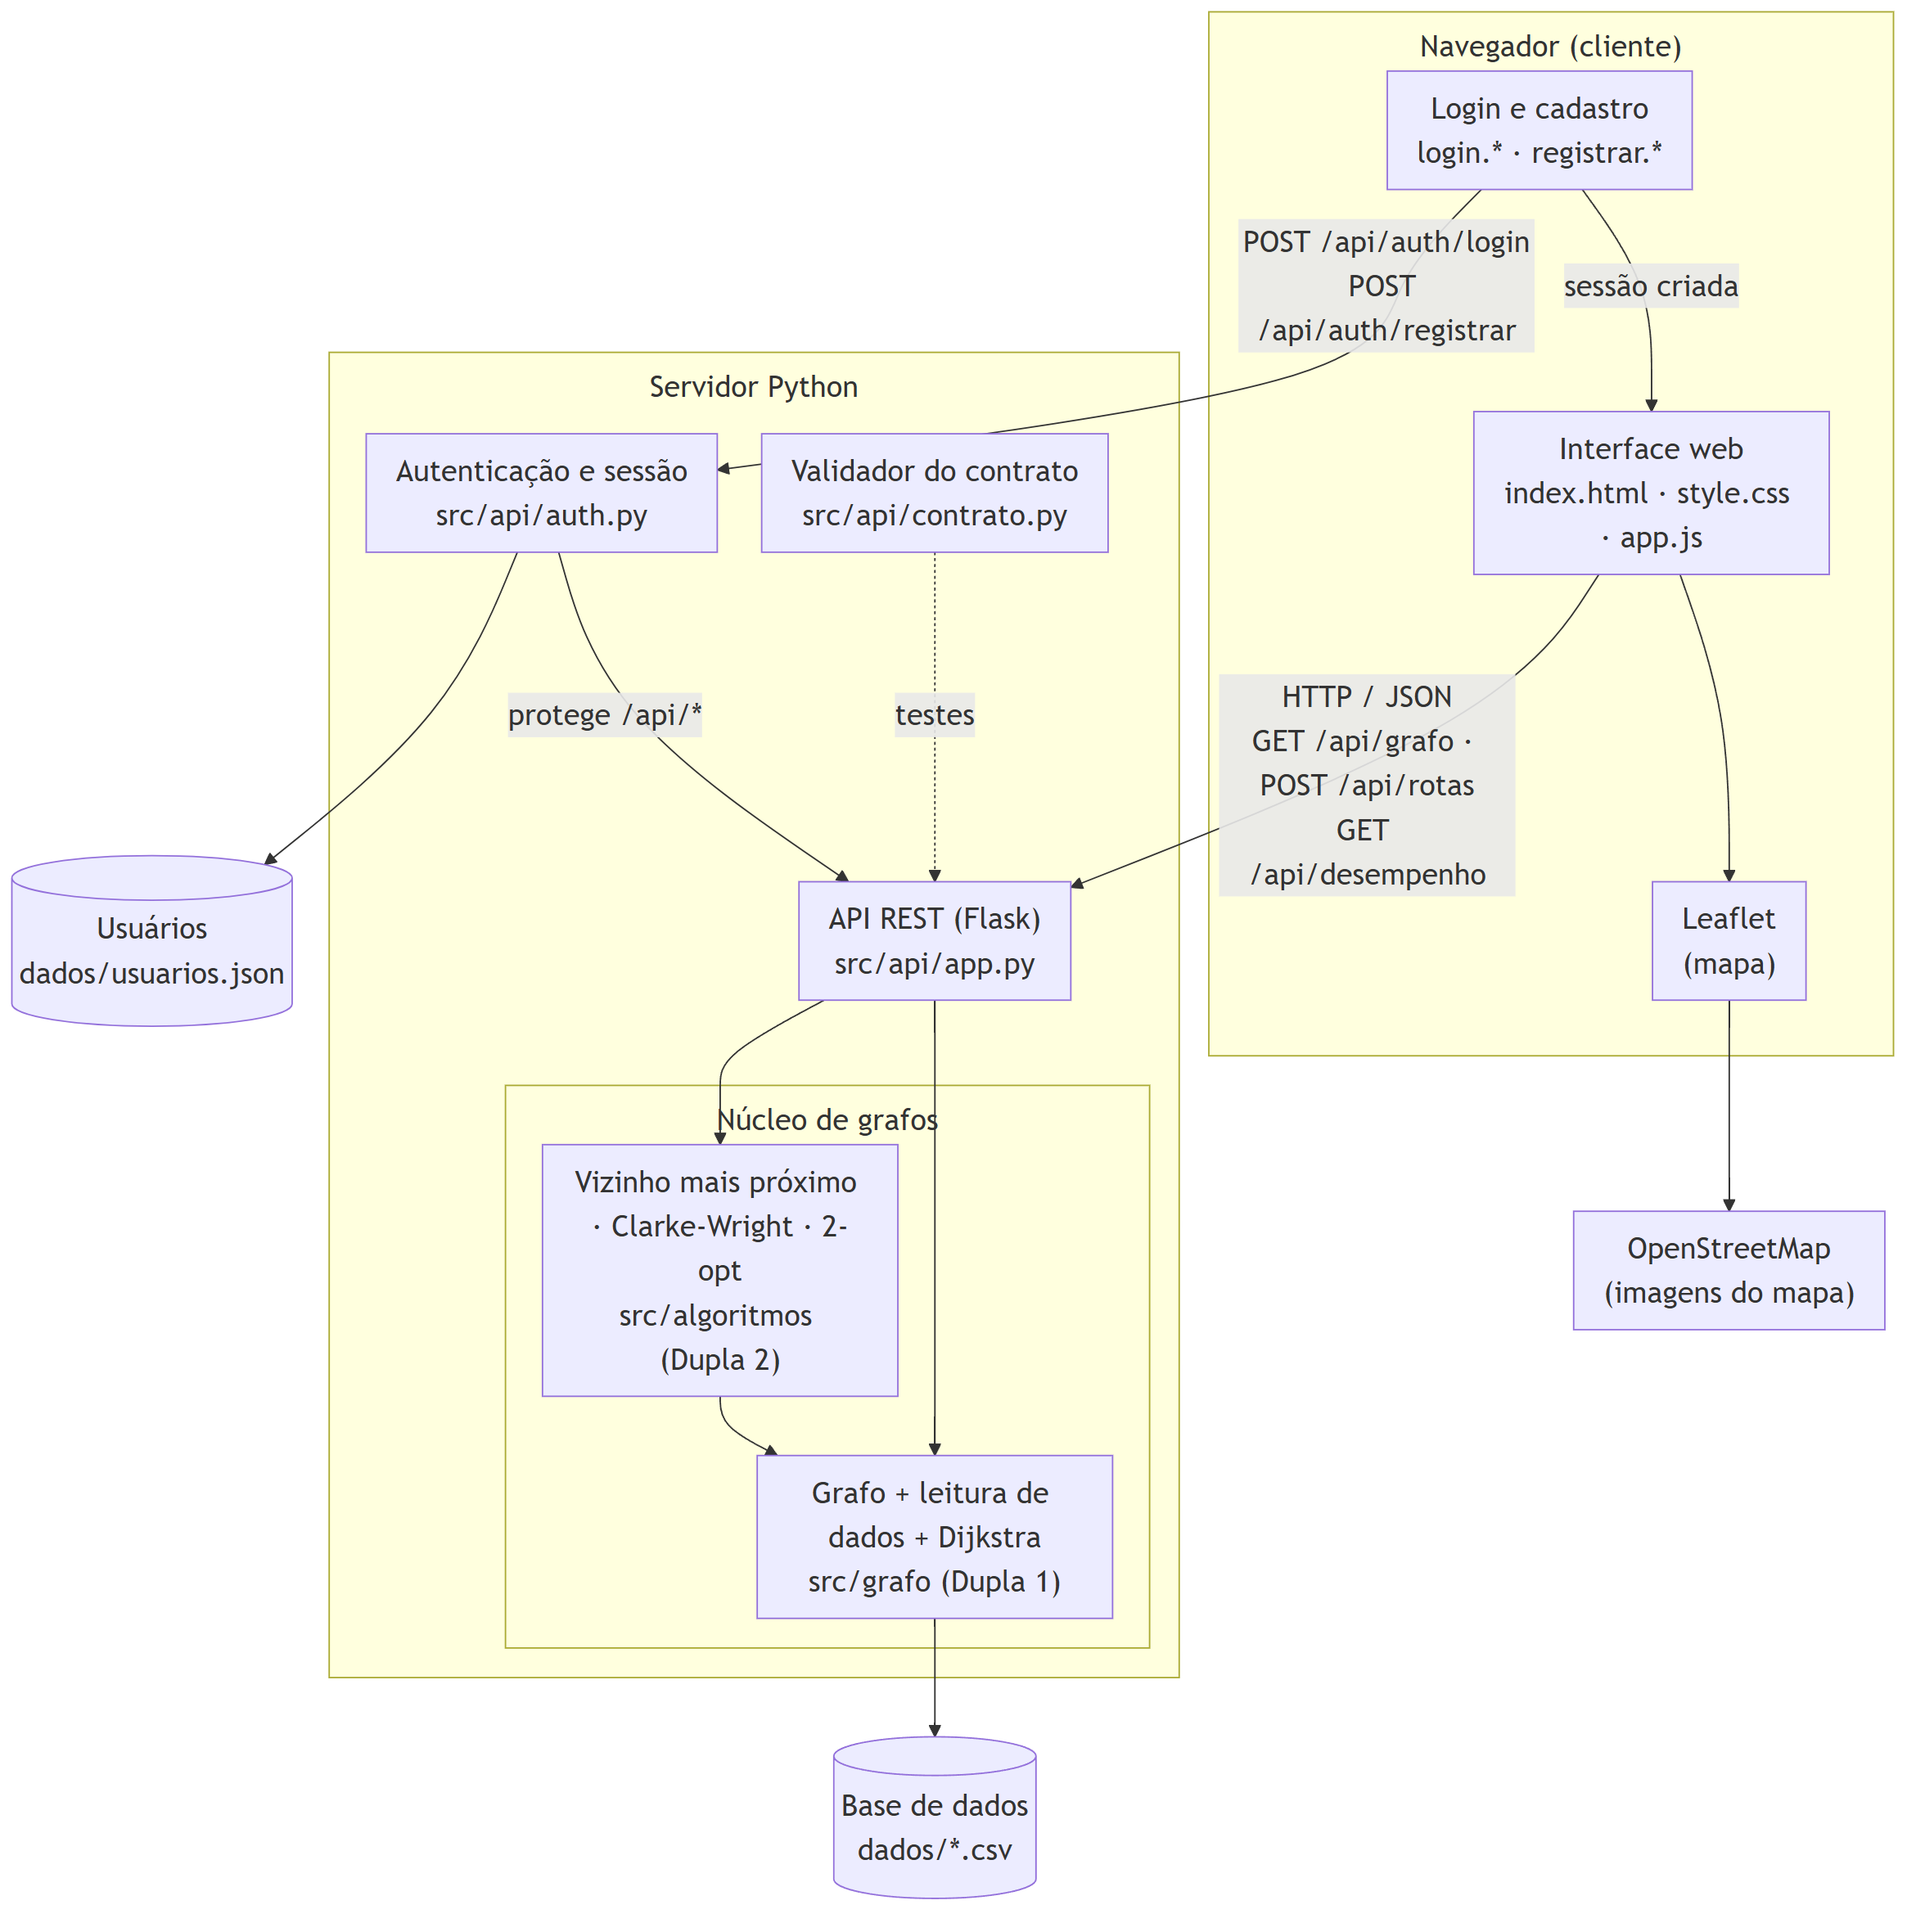
\includegraphics[width=.85\textwidth]{figuras/uml-componentes.png}
  \caption{Diagrama de componentes do RotaGrafo.}
  \label{fig:uml-componentes}
\end{figure}
\begin{figure}[H]
  \centering
  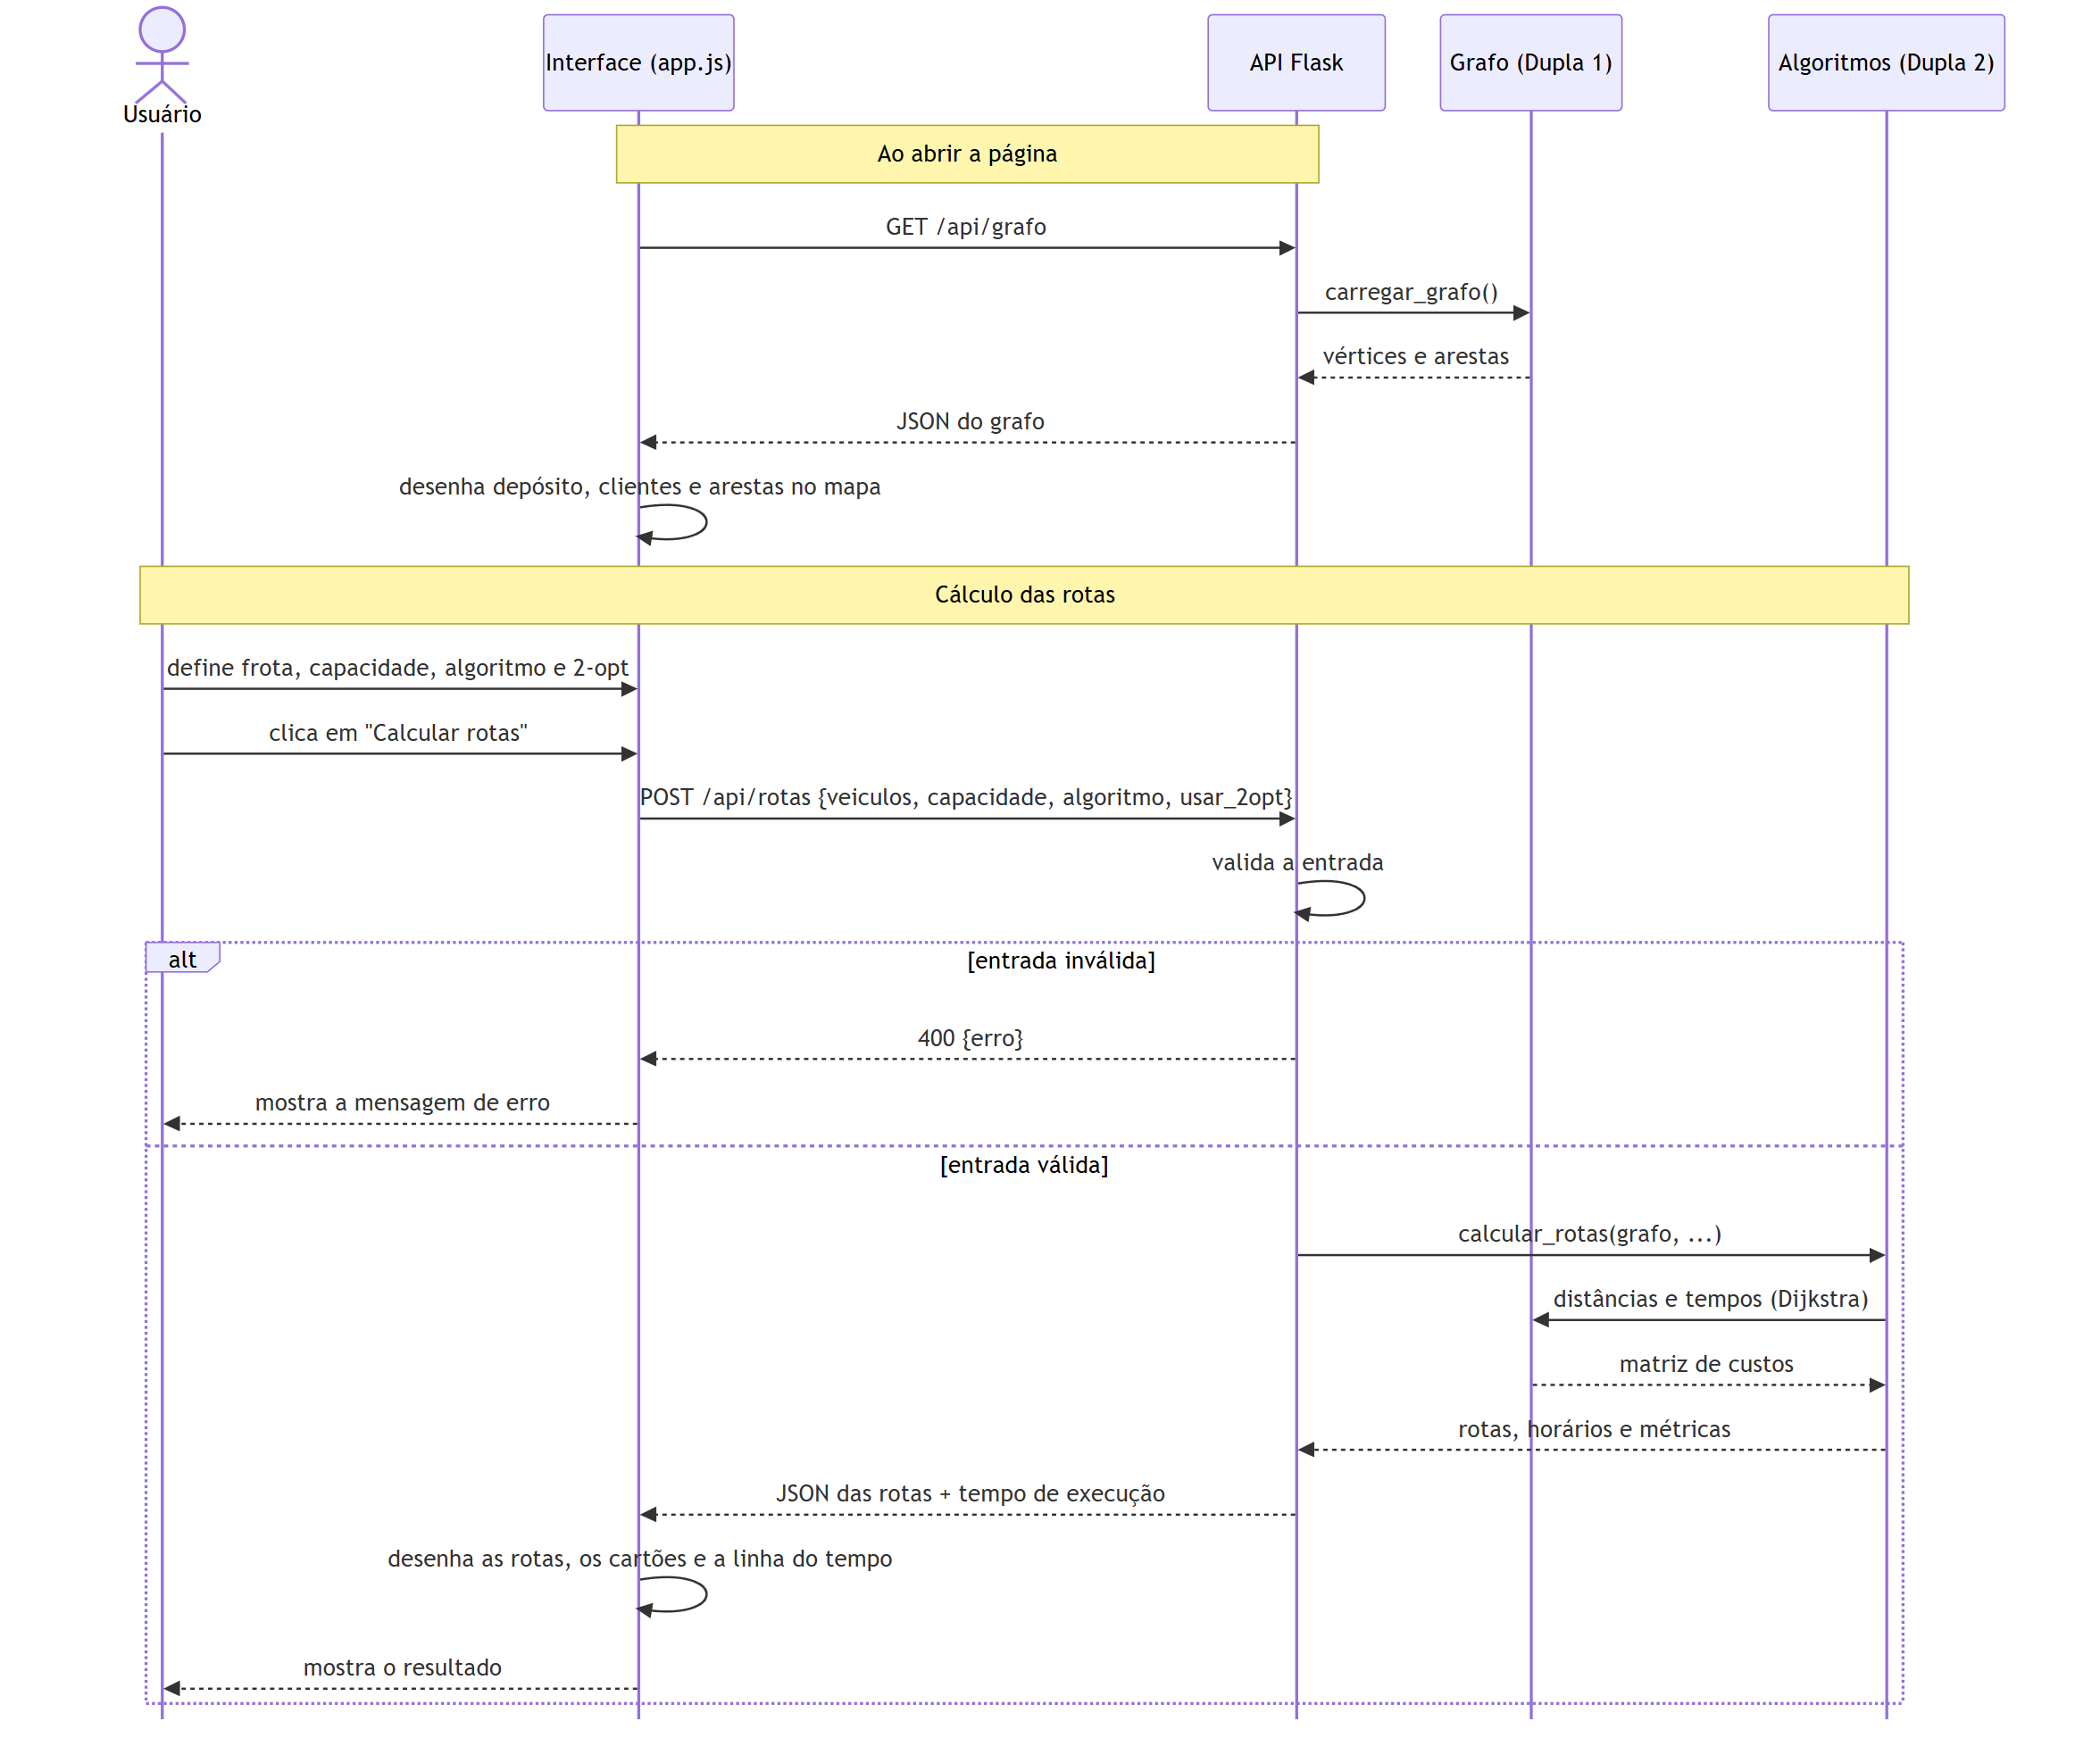
\includegraphics[width=\textwidth]{figuras/uml-sequencia.png}
  \caption{Diagrama de sequência do cálculo de rotas.}
  \label{fig:uml-sequencia}
\end{figure}
\begin{figure}[H]
  \centering
  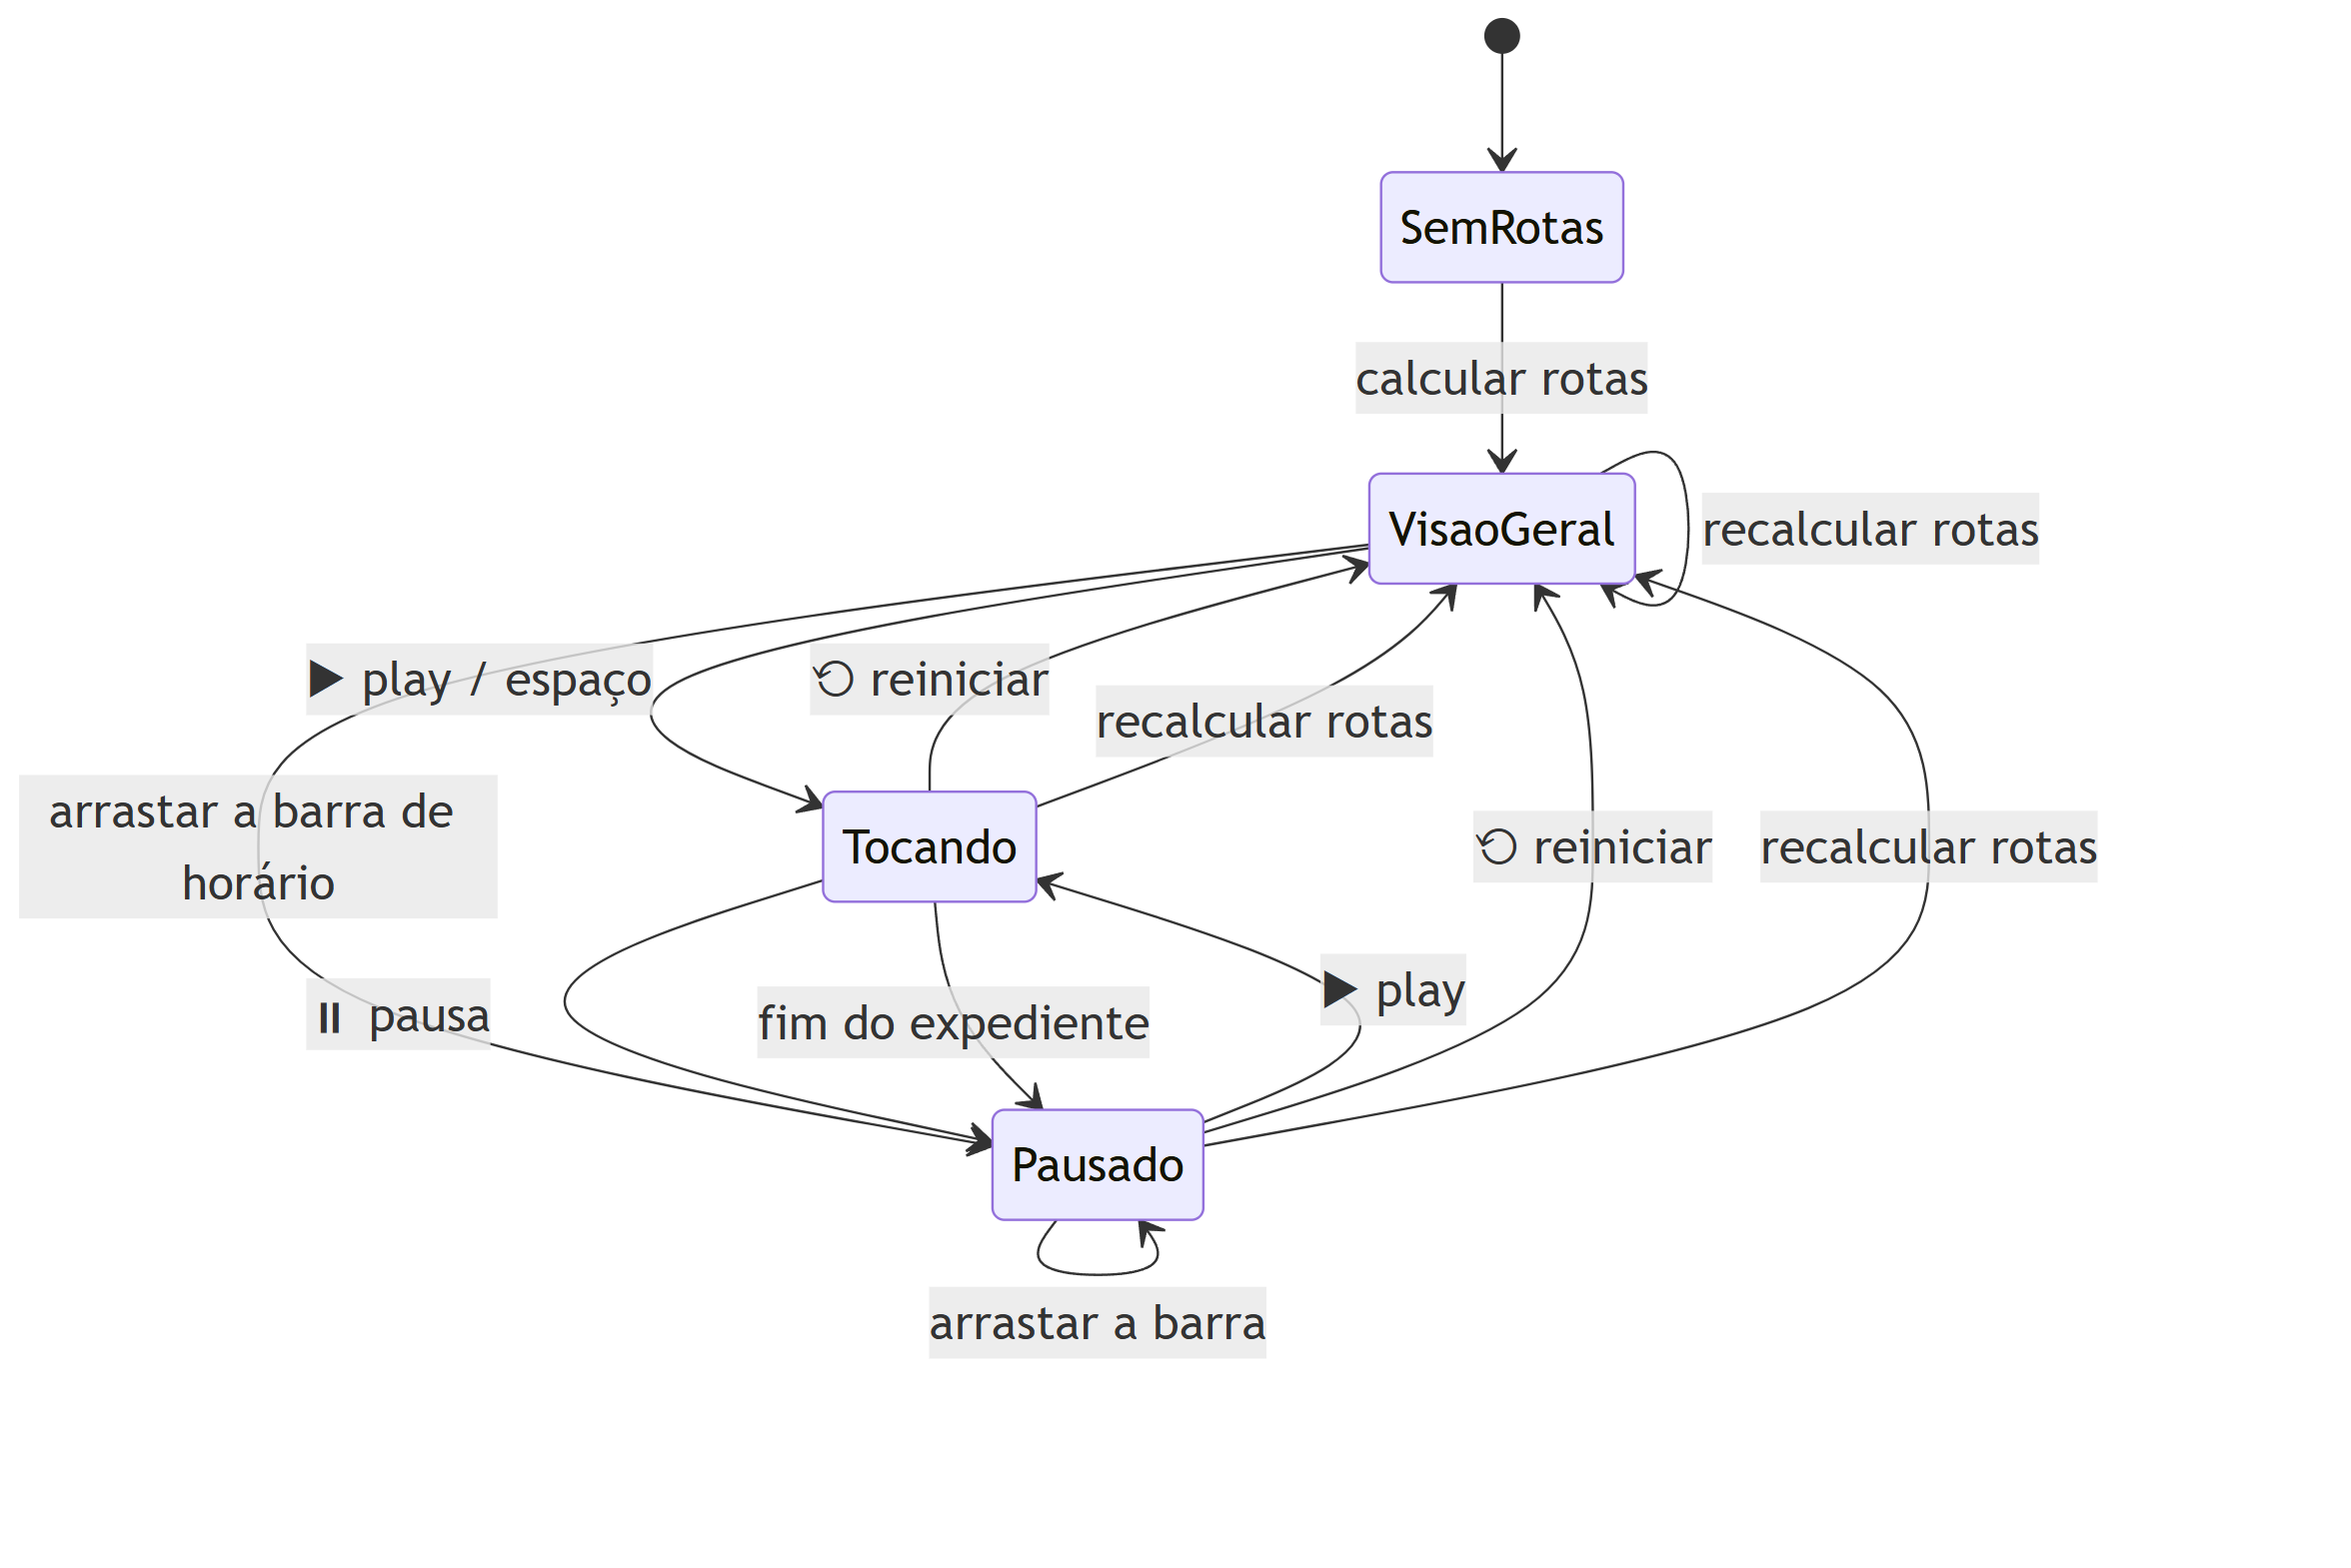
\includegraphics[width=.7\textwidth]{figuras/uml-estados-simulacao.png}
  \caption{Diagrama de estados da simulação.}
  \label{fig:uml-estados}
\end{figure}

% TODO: prints das telas (tirar com o sistema integrado)
% \begin{figure}[ht]
%   \centering
%   \includegraphics[width=\textwidth]{figuras/tela-principal.png}
%   \caption{Tela principal com as rotas calculadas.}
%   \label{fig:tela-principal}
% \end{figure}
% \begin{figure}[ht]
%   \centering
%   \includegraphics[width=\textwidth]{figuras/tela-simulacao.png}
%   \caption{Simulação do dia com a linha do tempo.}
%   \label{fig:tela-simulacao}
% \end{figure}
% \begin{figure}[ht]
%   \centering
%   \includegraphics[width=.6\textwidth]{figuras/tela-comparacao.png}
%   \caption{Comparação entre algoritmos.}
%   \label{fig:tela-comparacao}
% \end{figure}

% =====================================================================
\section{Resultados e Avaliação de Desempenho}\label{sec:resultados}
% [DUPLAS 1 e 2]

% TODO:
%  - instâncias usadas (tamanhos)
%  - tabela: algoritmo x distância total, veículos, atrasos, tempo de execução
%  - efeito do 2-opt (ganho percentual)
%  - gráfico de tempo de execução x número de vértices (validar a complexidade)
%  - comparação de desempenho com o NetworkX (Dupla 1)

% =====================================================================
\section{Limitações}\label{sec:limitacoes}
% [TODOS]

% Pontos de partida (ajustar ao que foi de fato implementado):
%  - heurísticas não garantem a solução ótima (o VRP é NP-difícil);
%  - distâncias estimadas por linha reta com fator de correção, não pela malha viária real;
%  - velocidade média constante (sem trânsito);
%  - frota homogênea e um único depósito;
%  - planejamento estático: não trata pedidos que chegam durante o dia.

% =====================================================================
\section{Conclusão}\label{sec:conclusao}
% [TODOS] — TODO

% =====================================================================
\section{Divisão de Responsabilidades}
% [DUPLA 3] — obrigatório pelo enunciado; ajustar ao que cada um fez de fato

\begin{table}[ht]
\centering
\caption{Responsabilidades de cada membro.}
\label{tab:responsabilidades}
\begin{tabular}{llp{7.5cm}}
\toprule
Dupla & Membro & Atividades \\
\midrule
1 & Zaine     & TODO \\
1 & Bruna     & TODO \\
2 & Kethellen & TODO \\
2 & Rafael    & TODO \\
3 & Filipe    & Interface web: mapa, rotas, simulação do dia, linha do tempo e guia de uso; relatório \\
3 & Vitor     & API Flask, contrato e testes de integração, aba de desempenho, diagramas UML da arquitetura; login, cadastro de contas e controle de sessão \\
\bottomrule
\end{tabular}
\end{table}

\bibliographystyle{sbc}
\bibliography{referencias}

\end{document}
